% !TeX TXS-program:compile = txs:///arara
% arara: lualatex: {shell: no, synctex: yes, interaction: batchmode}
% arara: pythontex: {rerun: always}
% arara: lualatex: {shell: no, synctex: yes, interaction: batchmode}
% arara: lualatex: {shell: no, synctex: yes, interaction: batchmode} if found('log', 'undefined references')

\documentclass[a4paper,11pt]{article}
\usepackage[pythontex]{cp-base}
%variables
\graphicspath{{./graphics/}}
\donnees[classe={1\up{ère} 2M2},matiere={[SPÉ.MATHS]},mois=Octobre,annee=2021,typedoc=QCM,numdoc=1]

%tableaux
\usepackage{booktabs}
\setlength\aboverulesep{0.65ex}
\setlength\belowrulesep{0.65ex}
\arrayrulecolor{titrebleu}

%formatage
\author{Pierquet}
\title{\nomfichier}
\hypersetup{pdfauthor={Pierquet},pdftitle={\nomfichier},allbordercolors=white,pdfborder=0 0 0,pdfstartview=FitH}
%divers
\lhead{\entete{\matiere}}
\chead{\entete{\lycee}}
\rhead{\entete{\classe{} - \mois{} \annee}}
\lfoot{\pied{\matiere}}
\cfoot{\logolycee}
\rfoot{\pied{\numeropagetot}}

%commandes pdfform
\renewcommand\LayoutCheckField[2]{#2~~#1}
\newcommand\choix[2]{%
	\raisebox{-.15\baselineskip}{\CheckBox[name=#1#2,width=1em,height=1em,bordercolor=black]{}}%
}
\newcommand\reponse[2]{%
	\raisebox{-.15\baselineskip}{\CheckBox[checkboxsymbol=\ding{95},color=red,name=#1#2,width=1em,height=1em,bordercolor=white]{}}%
}

\begin{document}

\pagestyle{fancy}

\begin{pycode}
def qcmalea(a,b,c,d):
	from random import shuffle
	reponses = [a,b,c,d]
	shuffle(reponses)
	return reponses

def qcmalea3(a,b,c):
	from random import shuffle
	reponses = [a,b,c]
	shuffle(reponses)
	return reponses

#Question1 - A
ENONCEQ1 = r"La forme canonique de $f(x)=-2x^2+4x+5$ est :"
Q1A = r"\reponse{R1}{A}\choix{Q1}{A}~"
Q1B = r"\reponse{R1}{B}\choix{Q1}{B}~"
Q1C = r"\reponse{R1}{C}\choix{Q1}{C}~"
Q1D = r"\reponse{R1}{D}\choix{Q1}{D}~"
Q1A += r"$-2(x-1)^2+7$"
Q1B += r"$-2(x+1)^2-7$"
Q1C += r"$(x-1)^2+7$"
Q1D += r"$(x+1)^2+7$"
reponsesQ1 = qcmalea(Q1A,Q1B,Q1C,Q1D)

#Question2 - A
ENONCEQ2 = r"On considère la fonction $g(x)=3x^2+6x-5$. On peut dire que $g$ admet :"
Q2A = r"\reponse{R2}{A}\choix{Q2}{A}~"
Q2B = r"\reponse{R2}{B}\choix{Q2}{B}~"
Q2C = r"\reponse{R2}{C}\choix{Q2}{C}~"
Q2D = r"\reponse{R2}{D}\choix{Q2}{D}~"
Q2A += r"comme minimum $-8$"
Q2B += r"comme maximum $-8$"
Q2C += r"comme minimum $-1$"
Q2D += r"comme maximum $-1$"
reponsesQ2 = qcmalea(Q2A,Q2B,Q2C,Q2D)

#Question3 - A
ENONCEQ3 = r"Les solutions de l'équation $2x^2+5x-3=0$ sont "
Q3A = r"\reponse{R3}{A}\choix{Q3}{A}~"
Q3B = r"\reponse{R3}{B}\choix{Q3}{B}~"
Q3C = r"\reponse{R3}{C}\choix{Q3}{C}~"
Q3D = r"\reponse{R3}{D}\choix{Q3}{D}~"
Q3A += r"$\mathscr{S}=\left\lbrace -3\,;\,\dfrac12 \right\rbrace$"
Q3B += r"$\mathscr{S}=\left\lbrace 3\,;\,-\dfrac12 \right\rbrace$"
Q3C += r"$\mathscr{S}=\left\lbrace 49 \right\rbrace$"
Q3D += r"$\mathscr{S}=\varnothing$"
reponsesQ3 = qcmalea(Q3A,Q3B,Q3C,Q3D)

#Question4 - A
ENONCEQ4 = r"Les solutions de l'équation $\dfrac{x+2}{x+1}=\dfrac{2x+3}{4}$ sont :"
Q4A = r"\reponse{R4}{A}\choix{Q4}{A}~"
Q4B = r"\reponse{R4}{B}\choix{Q4}{B}~"
Q4C = r"\reponse{R4}{C}\choix{Q4}{C}~"
Q4D = r"\reponse{R4}{D}\choix{Q4}{D}~"
Q4A += r"$\mathscr{S}=\left\lbrace \dfrac{-1+\sqrt{41}}{4}\,;\,\dfrac{-1-\sqrt{41}}{4} \right\rbrace$"
Q4B += r"$\mathscr{S}=\left\lbrace \dfrac{1+\sqrt{41}}{4}\,;\,\dfrac{1-\sqrt{41}}{4} \right\rbrace$"
Q4C += r"$\mathscr{S}=\left\lbrace -1,85\,;\,1,35 \right\rbrace$"
Q4D += r"$\mathscr{S}=\varnothing$"
reponsesQ4 = qcmalea(Q4A,Q4B,Q4C,Q4D)

#Question5 - A
ENONCEQ5 = r"On considère la suite $\suiten$ définie par $u_n = \dfrac{n}{n+1}+1$ pour tout entier naturel $n$. Le dixième terme de $\suiten$ vaut :"
Q5A = r"\reponse{R5}{A}\choix{Q5}{A}~"
Q5B = r"\reponse{R5}{B}\choix{Q5}{B}~"
Q5C = r"\reponse{R5}{C}\choix{Q5}{C}~"
Q5D = r"\reponse{R5}{D}\choix{Q5}{D}~"
Q5A += r"$1,9$"
Q5B += r"$1,909$"
Q5C += r"$1,8888$"
Q5D += r"$2$"
reponsesQ5 = qcmalea(Q5A,Q5B,Q5C,Q5D)

#Question6 - A
ENONCEQ6 = r"On considère la suite $\suiten[v]$ définie par $\begin{dcases} v_1 = 100 \\ v_{n+1}=0,75v_n+10\end{dcases}$ pour tout entier $n$. \\ On peut conjecturer que $\suiten[v]$ est :"
Q6A = r"\reponse{R6}{A}\choix{Q6}{A}~"
Q6B = r"\reponse{R6}{B}\choix{Q6}{B}~"
Q6C = r"\reponse{R6}{C}\choix{Q6}{C}~"
Q6D = r"\reponse{R6}{D}\choix{Q6}{D}~"
Q6A += r"décroissante et convergente vers 40"
Q6B += r"croissante et convergente vers 40"
Q6C += r"décroissante et divergente"
Q6D += r"croissante et divergente"
reponsesQ6 = qcmalea(Q6A,Q6B,Q6C,Q6D)

#Question7 - A
ENONCEQ7 = r"Soit $\suiten[w]$ la suite définie par $w_n=3n^2+2n-5$ pour tout entier $n$. une expression de $w_{n+1}$ est :"
Q7A = r"\reponse{R7}{A}\choix{Q7}{A}~"
Q7B = r"\reponse{R7}{B}\choix{Q7}{B}~"
Q7C = r"\reponse{R7}{C}\choix{Q7}{C}~"
Q7D = r"\reponse{R7}{D}\choix{Q7}{D}~"
Q7A += r"$3n^2+8n$"
Q7B += r"$3n^2+8n-2$"
Q7C += r"$3n^2+2n-4$"
Q7D += r"$3n^2+2n$"
reponsesQ7 = qcmalea(Q7A,Q7B,Q7C,Q7D)

#Question8 - A
ENONCEQ8 = r"On considère la suite $\suiten[t]$ définie par $\begin{dcases} t_0 = 10 \\ t_{n+1}=2t_n+n-4 \end{dcases}$ pour tout entier naturel $n$. \\ \bigskip La formule à rentrer dans la cellule \csheet{\helvbx B3} afin de calculer les termes consécutifs de $\suiten[t]$ par recopie est :"
Q8A = r"\reponse{R8}{A}\choix{Q8}{A}~"
Q8B = r"\reponse{R8}{B}\choix{Q8}{B}~"
Q8C = r"\reponse{R8}{C}\choix{Q8}{C}~"
Q8D = r"\reponse{R8}{D}\choix{Q8}{D}~"
Q8A += r"\csheet{\helvbx =2*B2+A2-4}"
Q8B += r"\csheet{\helvbx =2*B2+A3-4}"
Q8C += r"\csheet{\helvbx 2*B2+A2-4}"
Q8D += r"\csheet{\helvbx 2*B2+A3-4}"
reponsesQ8 = qcmalea(Q8A,Q8B,Q8C,Q8D)

#Question9 - A
ENONCEQ9 = r"Dans l'algorithme \calgpython{} suivant, que contient la variable \cpy{n} à la fin de son exécution ?"
Q9A = r"\reponse{R9}{A}\choix{Q9}{A}~"
Q9B = r"\reponse{R9}{B}\choix{Q9}{B}~"
Q9C = r"\reponse{R9}{C}\choix{Q9}{C}~"
Q9D = r"\reponse{R9}{D}\choix{Q9}{D}~"
Q9A += r"\cpy{86}"
Q9B += r"\cpy{85}"
Q9C += r"\cpy{10060,6965}"
Q9D += r"\cpy{0}"
reponsesQ9 = qcmalea(Q9A,Q9B,Q9C,Q9D)

#Question10 - A
ENONCEQ10 = r"On considère la suite $\suiten[z]$ dont le nuage de points est donné ci-dessous. Retrouver l'expression de $z_n$ en fonction de $n$ sachant que les points du nuage sont tous situés sur une même parabole."
Q10A = r"\reponse{R10}{A}\choix{Q10}{A}~"
Q10B = r"\reponse{R10}{B}\choix{Q10}{B}~"
Q10C = r"\reponse{R10}{C}\choix{Q10}{C}~"
Q10D = r"\reponse{R10}{D}\choix{Q10}{D}~"
Q10A += r"$z_n = 0,5n^2-2n-1$"
Q10B += r"$z_n = 2n+5$"
Q10C += r"$z_n = 0,5n^2+2n-1$"
Q10D += r"$z_n = n^2-2n-1$"
reponsesQ10 = qcmalea(Q10A,Q10B,Q10C,Q10D)
\end{pycode}

\part{Second degré, suites numériques}

\medskip

\begin{Form}

\textbf{\Large NOM Prénom : }~\raisebox{-.25\baselineskip}{\TextField[value=........................,width=10cm,height=2em,charsize=14pt,name=nomprenom,bordercolor=black]{}} \hfill~\textbf{\Large Note : }~\raisebox{-.25\baselineskip}{\TextField[width=2em,height=2em,charsize=14pt,name=note,bordercolor=black,color=1 0 0,align=1]{}}

\bigskip

\emph{Cet exercice est un questionnaire à choix multiple. Pour chacune des questions suivantes, \textbf{une seule} des quatre réponses proposées est exacte. Une bonne réponse rapporte un point. Une réponse fausse, une réponse multiple ou l’absence de réponse à une question ne rapporte ni n’enlève de point.\\
Pour répondre, compléter, à l'aide du logiciel {\small \red \textsf{Acrobat Reader} \faIcon[regular]{file-pdf}}, et déposer le document, renommé avec {\normalfont\cshell{\_ok}} à la fin, dans le répertoire {\normalfont\cshell{depot}} de votre espace personnel.}

\begin{enumerate}
	\item \py{ENONCEQ1}
	\begin{center}
		%\renewcommand{\arraystretch}{1.75}
		\begin{tabularx}{\linewidth}{@{}X@{}X@{}}
			\toprule
			\py{reponsesQ1[0]} & \py{reponsesQ1[1]} \\ \midrule
			\py{reponsesQ1[2]} & \py{reponsesQ1[3]} \\ \bottomrule
		\end{tabularx}
	\end{center}
	\item \py{ENONCEQ2}
	\begin{center}
		%\renewcommand{\arraystretch}{1.75}
		\begin{tabularx}{\linewidth}{@{}X@{}X@{}}
			\toprule
			\py{reponsesQ2[0]} & \py{reponsesQ2[1]} \\ \midrule
			\py{reponsesQ2[2]} & \py{reponsesQ2[3]} \\ \bottomrule
		\end{tabularx}
	\end{center}
	\item \py{ENONCEQ3}
	\begin{center}
		%\renewcommand{\arraystretch}{1.75}
		\begin{tabularx}{\linewidth}{@{}X@{}X@{}}
			\toprule
			\py{reponsesQ3[0]} & \py{reponsesQ3[1]} \\ \midrule
			\py{reponsesQ3[2]} & \py{reponsesQ3[3]} \\ \bottomrule
		\end{tabularx}
	\end{center}
	\item \py{ENONCEQ4}
	\begin{center}
		%\renewcommand{\arraystretch}{1.75}
		\begin{tabularx}{\linewidth}{@{}X@{}X@{}}
			\toprule
			\py{reponsesQ4[0]} & \py{reponsesQ4[1]} \\ \midrule
			\py{reponsesQ4[2]} & \py{reponsesQ4[3]} \\ \bottomrule
		\end{tabularx}
	\end{center}
	\item \py{ENONCEQ5}
	\begin{center}
		%\renewcommand{\arraystretch}{1.75}
		\begin{tabularx}{\linewidth}{@{}X@{}X@{}}
			\toprule
			\py{reponsesQ5[0]} & \py{reponsesQ5[1]} \\ \midrule
			\py{reponsesQ5[2]} & \py{reponsesQ5[3]} \\ \bottomrule
		\end{tabularx}
	\end{center}
	\item \py{ENONCEQ6}
	\begin{center}
		%\renewcommand{\arraystretch}{1.75}
		\begin{tabularx}{\linewidth}{@{}X@{}X@{}}
			\toprule
			\py{reponsesQ6[0]} & \py{reponsesQ6[1]} \\ \midrule
			\py{reponsesQ6[2]} & \py{reponsesQ6[3]} \\ \bottomrule
		\end{tabularx}
	\end{center}

	\newpage
	
	\item \py{ENONCEQ7}
	\begin{center}
		%\renewcommand{\arraystretch}{1.75}
		\begin{tabularx}{\linewidth}{@{}X@{}X@{}}
			\toprule
			\py{reponsesQ7[0]} & \py{reponsesQ7[1]} \\ \midrule
			\py{reponsesQ7[2]} & \py{reponsesQ7[3]} \\ \bottomrule
		\end{tabularx}
	\end{center}
	\item \py{ENONCEQ8}
	%
	\begin{center}
		\begin{tikzpicture}
			\tableur*[4]{A/4cm,B/4cm}
			%L1
			\celtxt[c]{A}{1}{n}
			\celtxt[c]{B}{1}{t\_n}
			%L2
			\celtxt[c]{A}{2}{0}
			\celtxt[c]{B}{2}{10}
			%L3
			\celtxt[c]{A}{3}{1}
			\selecCell{B}{3}
			%L4
			\celtxt[c]{A}{4}{2}
		\end{tikzpicture}
	\end{center}
	\begin{center}
		%\renewcommand{\arraystretch}{1.75}
		\begin{tabularx}{\linewidth}{@{}X@{}X@{}}
			\toprule
			\py{reponsesQ8[0]} & \py{reponsesQ8[1]} \\ \midrule
			\py{reponsesQ8[2]} & \py{reponsesQ8[3]} \\ \bottomrule
		\end{tabularx}
	\end{center}
	\item \py{ENONCEQ9}
	
	\begin{envpython}[10cm]
		n = 0
		u = 100
		while u < 10000 :
			n = n+1
			u = 1.05*u+3
	\end{envpython}
	\begin{center}
		%\renewcommand{\arraystretch}{1.75}
		\begin{tabularx}{\linewidth}{@{}X@{}X@{}}
			\toprule
			\py{reponsesQ9[0]} & \py{reponsesQ9[1]} \\ \midrule
			\py{reponsesQ9[2]} & \py{reponsesQ9[3]} \\ \bottomrule
		\end{tabularx}
	\end{center}
	\item \py{ENONCEQ10}
	
	\begin{center}
		\tunits{1}{1}
		\tdefgrille{0}{5}{1}{0.5}{-3}{2}{1}{0.5}
		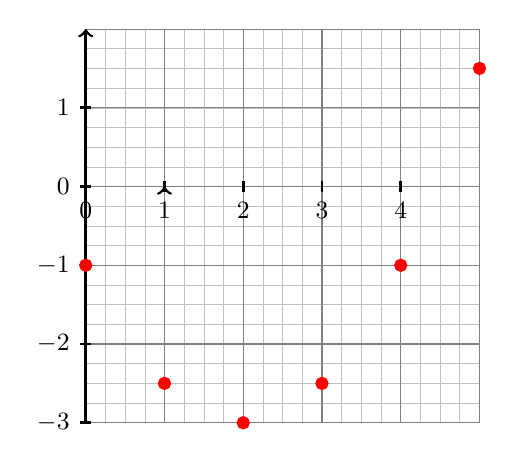
\begin{tikzpicture}
			%suite 0,5n^2-2n-1
			\draw [step=0.25,very thin,lightgray] (0,-3) grid (5,2) ;
			\draw [thin,gray] (0,-3) grid (5,2) ;
			\draw [line width=1pt,->] (\xmin,0) -- (\xmax,0) ;
			\draw [line width=1pt,->] (0,-3) -- (0,2) ;
			\foreach \x in {0,...,4}
				\draw[line width=1pt] (\x,2pt) -- (\x,-2pt) node [below] {\small $\x$};
			\foreach \y in {-3,...,1}
				\draw[line width=1pt] (2pt,\y) -- (-2pt,\y) node [left] {\small $\y$};
			\foreach \Point in {(0,-1), (1,-2.5), (2,-3), (3,-2.5), (4,-1), (5,1.5)}
				\draw[thick,red] plot[mark=*,mark size=2pt] coordinates {\Point};
				%\node at \Point {\red \large $\bullet$};
		\end{tikzpicture}
	\end{center}
	
	\begin{center}
		%\renewcommand{\arraystretch}{1.75}
		\begin{tabularx}{\linewidth}{@{}X@{}X@{}}
			\toprule
			\py{reponsesQ10[0]} & \py{reponsesQ10[1]} \\ \midrule
			\py{reponsesQ10[2]} & \py{reponsesQ10[3]} \\ \bottomrule
		\end{tabularx}
	\end{center}
\end{enumerate}

\end{Form}

\end{document}